\documentclass[9pt,twocolumn,twoside,]{pnas-new}

% Use the lineno option to display guide line numbers if required.
% Note that the use of elements such as single-column equations
% may affect the guide line number alignment.


\usepackage[T1]{fontenc}
\usepackage[utf8]{inputenc}
% Pandoc syntax highlighting
\usepackage{color}
\usepackage{fancyvrb}
\newcommand{\VerbBar}{|}
\newcommand{\VERB}{\Verb[commandchars=\\\{\}]}
\DefineVerbatimEnvironment{Highlighting}{Verbatim}{commandchars=\\\{\}}
% Add ',fontsize=\small' for more characters per line
\usepackage{framed}
\definecolor{shadecolor}{RGB}{248,248,248}
\newenvironment{Shaded}{\begin{snugshade}}{\end{snugshade}}
\newcommand{\AlertTok}[1]{\textcolor[rgb]{0.94,0.16,0.16}{#1}}
\newcommand{\AnnotationTok}[1]{\textcolor[rgb]{0.56,0.35,0.01}{\textbf{\textit{#1}}}}
\newcommand{\AttributeTok}[1]{\textcolor[rgb]{0.13,0.29,0.53}{#1}}
\newcommand{\BaseNTok}[1]{\textcolor[rgb]{0.00,0.00,0.81}{#1}}
\newcommand{\BuiltInTok}[1]{#1}
\newcommand{\CharTok}[1]{\textcolor[rgb]{0.31,0.60,0.02}{#1}}
\newcommand{\CommentTok}[1]{\textcolor[rgb]{0.56,0.35,0.01}{\textit{#1}}}
\newcommand{\CommentVarTok}[1]{\textcolor[rgb]{0.56,0.35,0.01}{\textbf{\textit{#1}}}}
\newcommand{\ConstantTok}[1]{\textcolor[rgb]{0.56,0.35,0.01}{#1}}
\newcommand{\ControlFlowTok}[1]{\textcolor[rgb]{0.13,0.29,0.53}{\textbf{#1}}}
\newcommand{\DataTypeTok}[1]{\textcolor[rgb]{0.13,0.29,0.53}{#1}}
\newcommand{\DecValTok}[1]{\textcolor[rgb]{0.00,0.00,0.81}{#1}}
\newcommand{\DocumentationTok}[1]{\textcolor[rgb]{0.56,0.35,0.01}{\textbf{\textit{#1}}}}
\newcommand{\ErrorTok}[1]{\textcolor[rgb]{0.64,0.00,0.00}{\textbf{#1}}}
\newcommand{\ExtensionTok}[1]{#1}
\newcommand{\FloatTok}[1]{\textcolor[rgb]{0.00,0.00,0.81}{#1}}
\newcommand{\FunctionTok}[1]{\textcolor[rgb]{0.13,0.29,0.53}{\textbf{#1}}}
\newcommand{\ImportTok}[1]{#1}
\newcommand{\InformationTok}[1]{\textcolor[rgb]{0.56,0.35,0.01}{\textbf{\textit{#1}}}}
\newcommand{\KeywordTok}[1]{\textcolor[rgb]{0.13,0.29,0.53}{\textbf{#1}}}
\newcommand{\NormalTok}[1]{#1}
\newcommand{\OperatorTok}[1]{\textcolor[rgb]{0.81,0.36,0.00}{\textbf{#1}}}
\newcommand{\OtherTok}[1]{\textcolor[rgb]{0.56,0.35,0.01}{#1}}
\newcommand{\PreprocessorTok}[1]{\textcolor[rgb]{0.56,0.35,0.01}{\textit{#1}}}
\newcommand{\RegionMarkerTok}[1]{#1}
\newcommand{\SpecialCharTok}[1]{\textcolor[rgb]{0.81,0.36,0.00}{\textbf{#1}}}
\newcommand{\SpecialStringTok}[1]{\textcolor[rgb]{0.31,0.60,0.02}{#1}}
\newcommand{\StringTok}[1]{\textcolor[rgb]{0.31,0.60,0.02}{#1}}
\newcommand{\VariableTok}[1]{\textcolor[rgb]{0.00,0.00,0.00}{#1}}
\newcommand{\VerbatimStringTok}[1]{\textcolor[rgb]{0.31,0.60,0.02}{#1}}
\newcommand{\WarningTok}[1]{\textcolor[rgb]{0.56,0.35,0.01}{\textbf{\textit{#1}}}}

% tightlist command for lists without linebreak
\providecommand{\tightlist}{%
  \setlength{\itemsep}{0pt}\setlength{\parskip}{0pt}}


% Pandoc citation processing
%From Pandoc 3.1.8
% definitions for citeproc citations
\NewDocumentCommand\citeproctext{}{}
\NewDocumentCommand\citeproc{mm}{%
  \begingroup\def\citeproctext{#2}\cite{#1}\endgroup}
\makeatletter
 % allow citations to break across lines
 \let\@cite@ofmt\@firstofone
 % avoid brackets around text for \cite:
 \def\@biblabel#1{}
 \def\@cite#1#2{{#1\if@tempswa , #2\fi}}
\makeatother
\newlength{\cslhangindent}
\setlength{\cslhangindent}{1.5em}
\newlength{\csllabelwidth}
\setlength{\csllabelwidth}{3em}
\newenvironment{CSLReferences}[2] % #1 hanging-indent, #2 entry-spacing
 {\begin{list}{}{%
  \setlength{\itemindent}{0pt}
  \setlength{\leftmargin}{0pt}
  \setlength{\parsep}{0pt}
  % turn on hanging indent if param 1 is 1
  \ifodd #1
   \setlength{\leftmargin}{\cslhangindent}
   \setlength{\itemindent}{-1\cslhangindent}
  \fi
  % set entry spacing
  \setlength{\itemsep}{#2\baselineskip}}}
 {\end{list}}
\usepackage{calc}
\newcommand{\CSLBlock}[1]{#1\hfill\break}
\newcommand{\CSLLeftMargin}[1]{\parbox[t]{\csllabelwidth}{#1}}
\newcommand{\CSLRightInline}[1]{\parbox[t]{\linewidth - \csllabelwidth}{#1}\break}
\newcommand{\CSLIndent}[1]{\hspace{\cslhangindent}#1}

\providecommand{\pandocbounded}[1]{#1}
\usepackage{graphicx}
\usepackage{amsmath}
\usepackage{amsfonts}
\usepackage{amssymb}
\usepackage{bbm}
\usepackage{algorithm}
\usepackage{algpseudocode}
\DeclareMathOperator*{\argmin}{argmin}
\DeclareMathOperator*{\argmax}{argmax}
\DeclareMathOperator\diag{diag}
\renewcommand{\algorithmicrequire}{\textbf{Input:}}
\renewcommand{\algorithmicensure}{\textbf{Output:}}

\templatetype{pnasresearcharticle}  % Choose template

\title{Survival driven deconvolution (deSurv) reveals clinically
relevant tumor and stromal gene signatures}

\author[a,1,2]{Amber Young}
\author[b]{Alisa}
\author[a]{Didong}
\author[a,c]{Naim}

  \affil[a]{University of North Carolina at Chapel Hill, Department,
Street, City, State, Zip}
  \affil[b]{Another University Department, Street, City, State, Zip}


% Please give the surname of the lead author for the running footer
\leadauthor{Anonymous}

% Please add here a significance statement to explain the relevance of your work
\significancestatement{Authors must submit a 120-word maximum statement
about the significance of their research paper written at a level
understandable to an undergraduate educated scientist outside their
field of speciality. The primary goal of the Significance Statement is
to explain the relevance of the work in broad context to a broad
readership. The Significance Statement appears in the paper itself and
is required for all research papers.}


\authorcontributions{Please provide details of author contributions
here.}

\authordeclaration{Please declare any conflict of interest here.}


\correspondingauthor{\textsuperscript{2} To whom correspondence should
be addressed. E-mail:
\href{mailto:bob@email.com}{\nolinkurl{bob@email.com}}}

% Keywords are not mandatory, but authors are strongly encouraged to provide them. If provided, please include two to five keywords, separated by the pipe symbol, e.g:
 \keywords{  one |  two |  optional |  optional |  optional  } 

\begin{abstract}
Molecular subtyping in cancer is an ongoing problem that relies on the
identification of robust and replicable gene signatures. While
transcriptomic profiling has revealed recurrent gene expression patterns
in various types of cancer, the prognostic value of these signatures is
typically evaluated in retrospect. This is due to the reliance on
unsupervised learning methods for identifying cell-type-specific signals
and clustering patients into molecular subtypes. Here we present a
Survival-driven Deconvolution tool (deSurv) that integrates bulk
RNA-sequencing data with patient survival information to identify
cell-type-enriched gene signatures associated with prognosis. Applying
deSurv to various cohorts in pancreatic, bladder, and colorectal cancer,
we uncover previously unrecognized gene signatures linked to tumor,
stromal, and immune compartments, including … Several identified
signatures exhibit consistent prognostic value across cohorts and cancer
types and demonstrate potential as therapeutic targets or biomarkers.
Our approach highlights the value of using patient outcomes during gene
signature discovery.
\end{abstract}

\dates{This manuscript was compiled on \today}
\doi{\url{www.pnas.org/cgi/doi/10.1073/pnas.XXXXXXXXXX}}

\begin{document}

% Optional adjustment to line up main text (after abstract) of first page with line numbers, when using both lineno and twocolumn options.
% You should only change this length when you've finalised the article contents.
\verticaladjustment{-2pt}



\maketitle
\thispagestyle{firststyle}
\ifthenelse{\boolean{shortarticle}}{\ifthenelse{\boolean{singlecolumn}}{\abscontentformatted}{\abscontent}}{}

% If your first paragraph (i.e. with the \dropcap) contains a list environment (quote, quotation, theorem, definition, enumerate, itemize...), the line after the list may have some extra indentation. If this is the case, add \parshape=0 to the end of the list environment.

\acknow{Please include your acknowledgments here, set in a single
paragraph. Please do not include any acknowledgments in the Supporting
Information, or anywhere else in the manuscript.}

Molecular subtyping has become a cornerstone of precision oncology,
enabling the stratification of cancer patients based on distinct gene
expression patterns. This stratification informs prognosis, guides
therapeutic decisions, and enhances our understanding of tumor biology.
However, despite considerable progress, current approaches often depend
on unsupervised learning techniques, which may not reliably capture the
prognostic relevance of specific cell-type contributions. As a result,
many proposed gene expression signatures are evaluated retrospectively
for clinical relevance and may lack consistent replication across
independent cohorts and cancer types.

A key limitation lies in the disconnect between molecular subtyping and
clinical outcomes. Most methods do not explicitly incorporate survival
information during signature discovery, potentially overlooking gene
programs with true prognostic value. Moreover, the complex interplay
between malignant, stromal, and immune compartments in the tumor
microenvironment presents an additional challenge to disentangling
biologically meaningful and clinically actionable signals.

To address these issues, we developed deSurv, a Survival-driven
Deconvolution framework that integrates bulk RNA-sequencing data with
patient survival outcomes to uncover cell-type-enriched gene signatures
with prognostic relevance. By aligning molecular signals with clinical
endpoints, deSurv provides a more targeted and interpretable approach to
gene signature discovery. Applying this method to diverse cancer
cohorts, we identify novel prognostic markers within tumor, stromal, and
immune compartments, offering new insights into the cellular basis of
patient outcomes and revealing candidates for biomarker development or
therapeutic intervention.

\section*{Results}\label{results}
\addcontentsline{toc}{section}{Results}

\subsection*{DeSurv incorporates patient survival information directly
into
deconvolution}\label{desurv-incorporates-patient-survival-information-directly-into-deconvolution}
\addcontentsline{toc}{subsection}{DeSurv incorporates patient survival
information directly into deconvolution}

We developed deSurv, a survival-driven deconvolution framework that
integrates bulk RNA-sequencing data with patient outcome information to
identify cell-type-enriched gene signatures with prognostic value.
Unlike standard unsupervised methods that cluster expression patterns
without regard to patient survival, deSurv incorporates time-to-event
data directly into the signature discovery process. We applied deSurv to
bulk RNA-seq profiles from pancreatic, bladder, and colorectal cancer
cohorts, each with matched clinical follow-up data, encompassing a total
of n = XXXX patients across discovery and validation sets (Table 1). An
overview of DeSurv can be found in Figure @ref(fig:fig-schema)

\begin{Shaded}
\begin{Highlighting}[]
\NormalTok{knitr}\SpecialCharTok{::}\FunctionTok{include\_graphics}\NormalTok{(}\StringTok{"desurv\_schematic\_v5.pdf"}\NormalTok{)}
\end{Highlighting}
\end{Shaded}

\begin{figure}
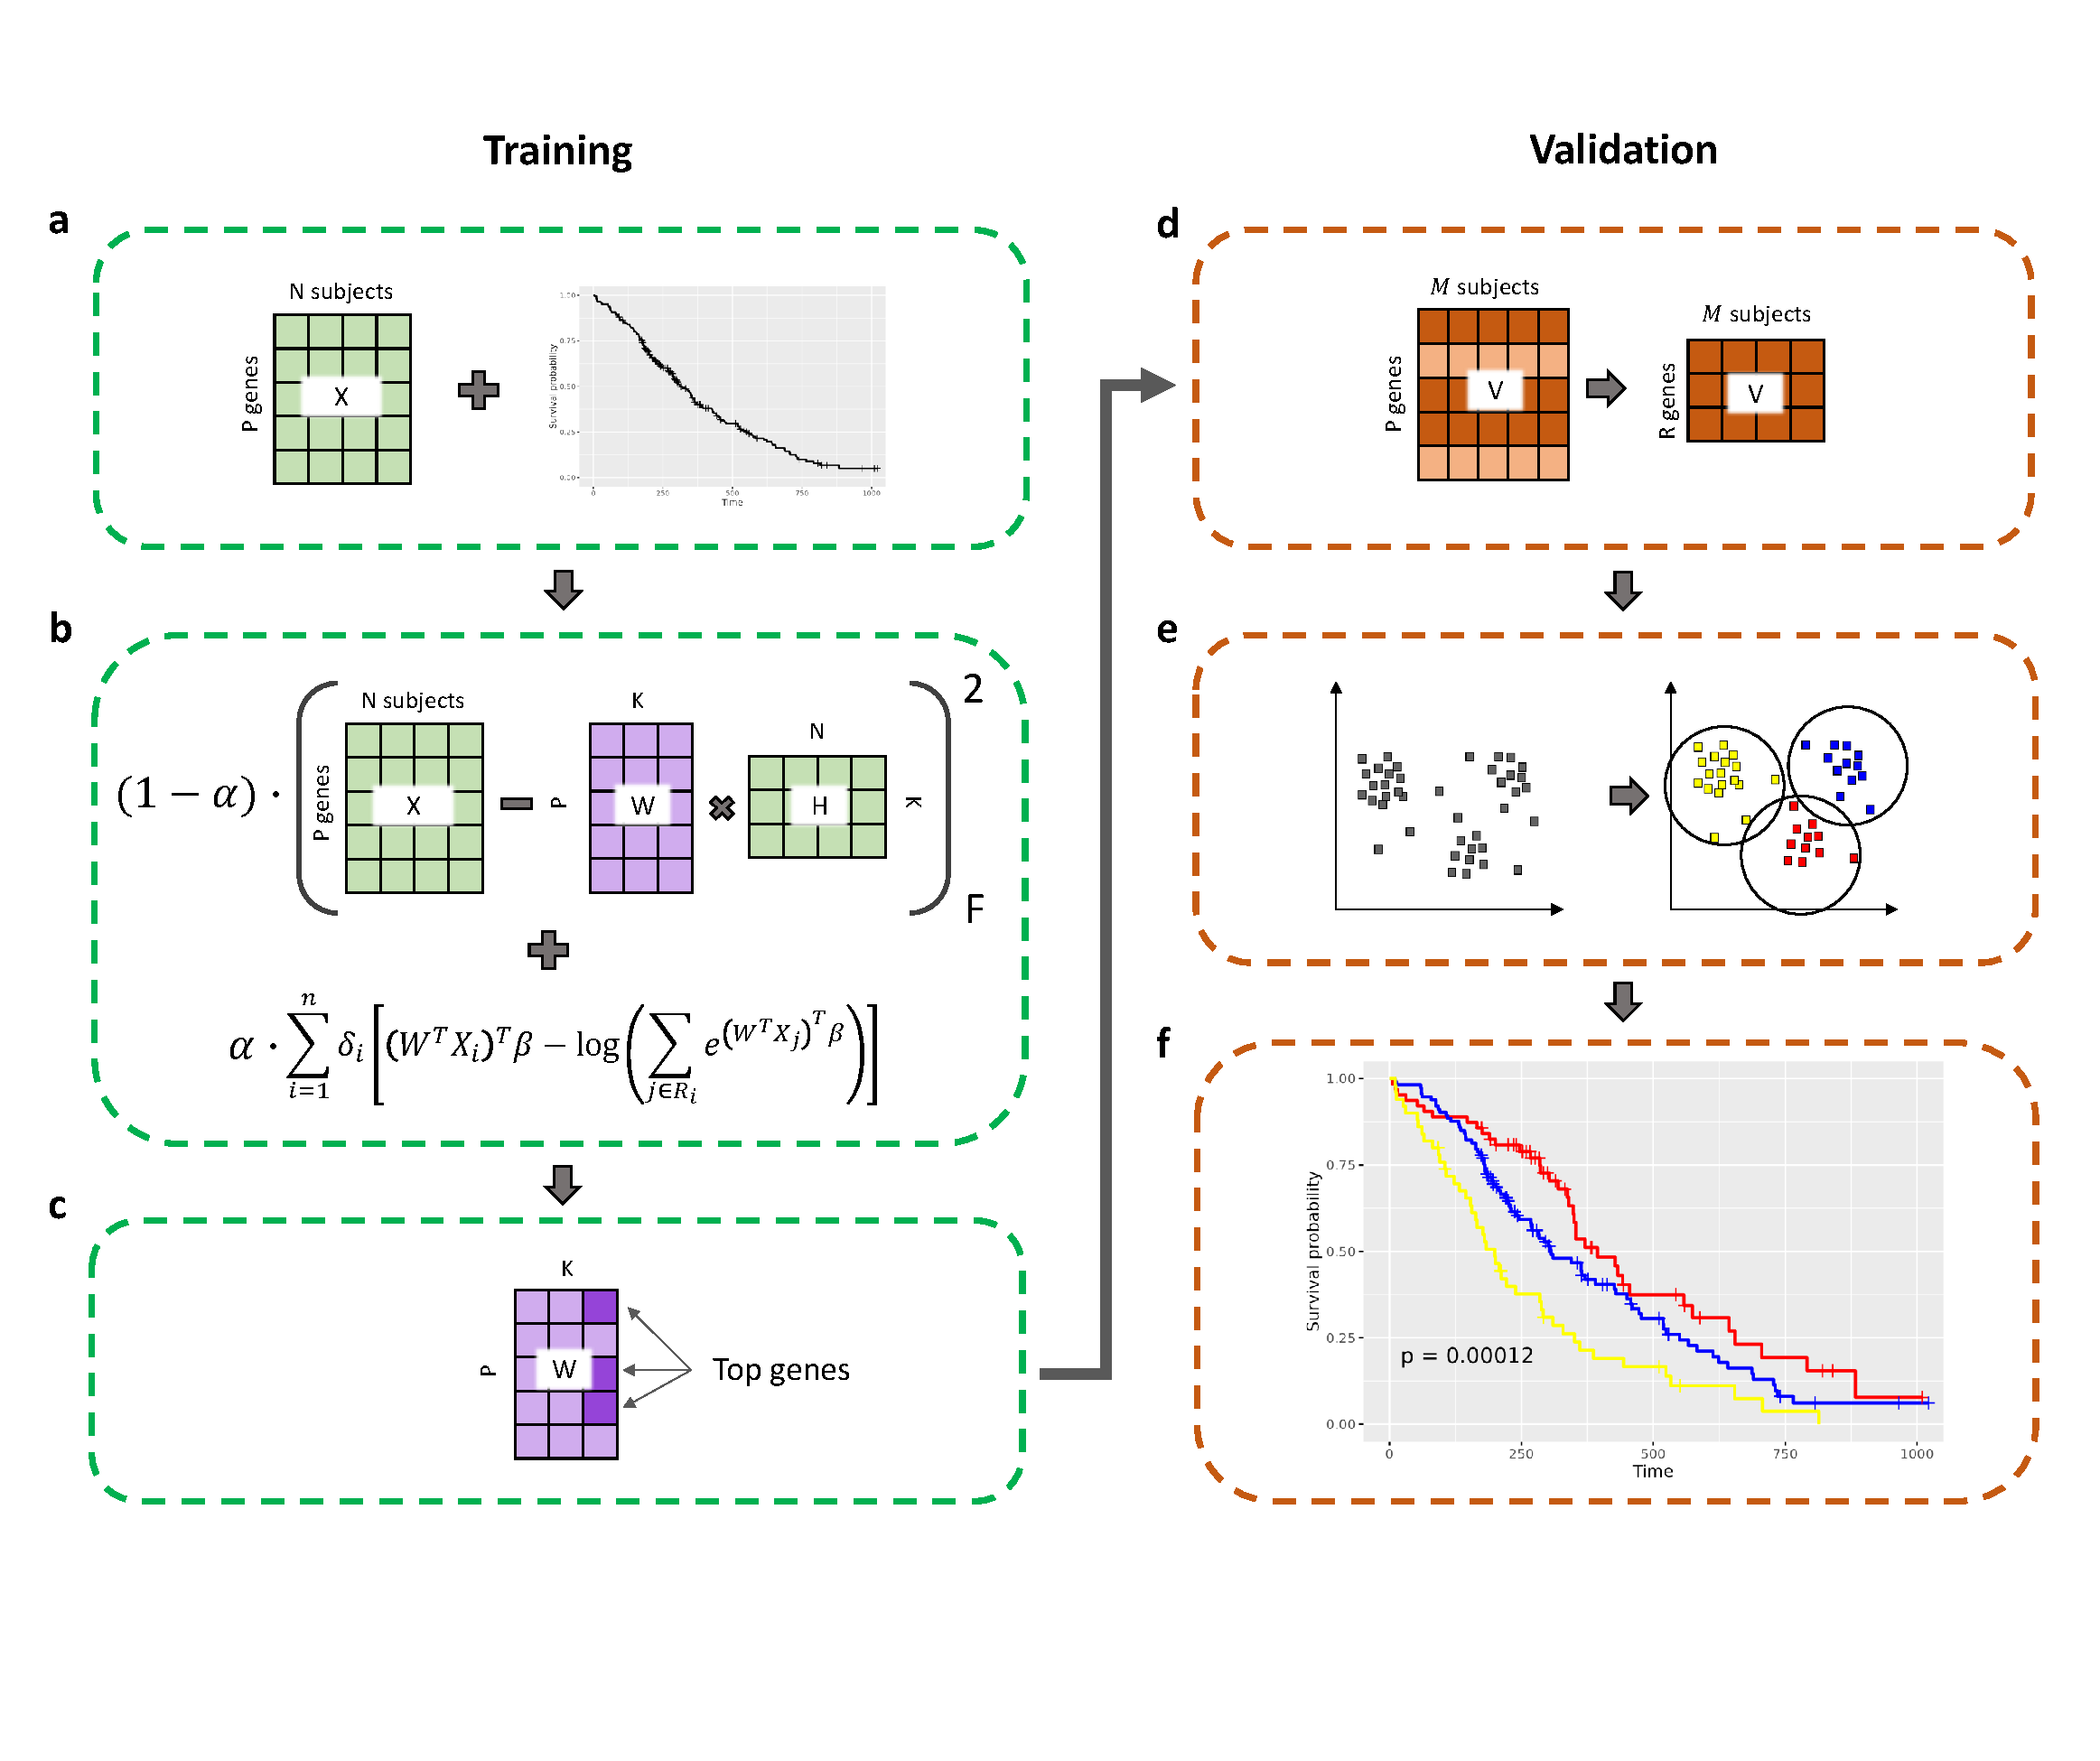
\includegraphics[width=0.8\linewidth]{desurv_schematic_v5} \caption{DeSurv overview}\label{fig:fig-schema}
\end{figure}

\subsection*{DeSurv captures distinct cell-type specific gene
signatures}\label{desurv-captures-distinct-cell-type-specific-gene-signatures}
\addcontentsline{toc}{subsection}{DeSurv captures distinct cell-type
specific gene signatures}

In PDAC, deSurv identified cell-type-specific signatures spanning tumor,
stromal, and immune compartments. Many signatures were distinct from
those obtained using unsupervised methods (Figure 2a and 2b).
Representative heatmaps illustrate the differential expression of these
signatures across patients (Figure 2c).

\subsection*{DeSurv extracts prognostic tumor
signatures}\label{desurv-extracts-prognostic-tumor-signatures}
\addcontentsline{toc}{subsection}{DeSurv extracts prognostic tumor
signatures}

Tumor signatures derived using deSurv stratified patients into groups
with significantly different survival outcomes (log-rank P \textless{}
0.001 in all datasets), often outperforming unsupervised methods
(Figures 3a-c). For example, a deSurv tumor signature achieved a
concordance index (C-index) of 0.72 compared to 0.61 for the nearest
unsupervised equivalent (Table 1). Performance gains were consistent in
independent validation cohorts (Figures 3d-e) , indicating that survival
integration during signature discovery enhances prognostic robustness.

\subsection*{DeSurv extracts prognostic stromal
factors}\label{desurv-extracts-prognostic-stromal-factors}
\addcontentsline{toc}{subsection}{DeSurv extracts prognostic stromal
factors}

Figure: Panel A , Panel B, Panel C,

At k=9, DeSurv finds an iCAF factor that is not found in standard NMF.
When we cluster on this factor in the validation datasets the resulting
clusters are prognostic for patient survival. Note that almost all other
stromal factors are not associated with survival.

\subsection*{Cross-cancer robustness of prognostic
signatures}\label{cross-cancer-robustness-of-prognostic-signatures}
\addcontentsline{toc}{subsection}{Cross-cancer robustness of prognostic
signatures}

Several deSurv-derived signatures retained prognostic value when applied
to other cancer types. A tumor signature discovered in PDAC was also
prognostic in colorectal cancer (log-rank P = xx), and a stromal
signature from pancreatic cancer predicted improved survival in bladder
cancer (Figure 4a). Heatmaps of hazard ratios across cross-cancer
applications revealed that X\% of signatures demonstrated statistically
significant associations in at least two cancer types (Figure 4b),
suggesting a degree of pan-cancer prognostic relevance.

\section*{Discussion}\label{discussion}
\addcontentsline{toc}{section}{Discussion}

\section*{Materials and methods}\label{materials-and-methods}
\addcontentsline{toc}{section}{Materials and methods}

\subsection*{Standard NMF}\label{standard-nmf}
\addcontentsline{toc}{subsection}{Standard NMF}

Let \(X\) be a bulk gene expression matrix of \(p\) genes by \(n\)
subjects. Standard NMF seeks to reconstruct X using two nonnegative
matrices \(W\) and \(H\) such that \(X = WH\), where \(W\) is a
\(p \times k\) matrix of gene weights and \(H\) is a \(k \times n\)
matrix of sample weights. This is done by minimizing the loss function

\begin{equation}
    ||X - WH||^2_F
\end{equation}

where \(F\) represents the Frobenius norm.

Multiplicative updates were proposed by Lee and Seung with the following
update rules (1):

\begin{equation}
    W_{ij} = \frac{W_{ij} (XH^T)_{ij}}{(WHH^T)_{ij}}
\end{equation}

\begin{equation}
    H_{ij} = H_{ij} \frac{(W^TX)_{ij}}{(W^TWH)_{ij}}
\end{equation}

These updates are alternated until convergence to a stationary point.

\subsection*{Proportional Hazards}\label{proportional-hazards}
\addcontentsline{toc}{subsection}{Proportional Hazards}

To determine how the lower dimensional representation of X is associated
with patient survival outcomes, we take \(Z=W^TX\) to be the covariates
passed to the proportional hazards model. The matrix \(Z\) can be
interpreted as the transformation of the data matrix \(X\) into the
lower dimensional space, such that \(Z_{ri}\) represents a score for the
contribution of factor \(r\) to subject \(i\).

Let \(y_i = \min(T_i,C_i)\) where \(T_i\) is the event time and \(C_i\)
is the censoring time for the \(i\)th subject; let \(\delta_i\)
represent the indicator that the event time for the \(i\)th subject is
observed. The the log partial likelihood is

\begin{equation}
    \ell(W,\beta) = \sum_{i=1}^n \delta_i \left[Z_i^T\beta - \log\left(\sum_{j=1}^n \exp \left(Z_j^T\beta\right) \mathbbm{1} (y_j \geq y_i) \right)\right]
\end{equation}

\subsection*{DeSurv}\label{desurv}
\addcontentsline{toc}{subsection}{DeSurv}

DeSurv is a semi-supervised extension of NMF that incorporates the cox
proportional hazards directly into the NMF model to encourage the
discovered factors to be associated with patient survival. We propose
the following loss function

\begin{equation}
    \mathcal{L}(W,H,\beta) = \frac{(1-\alpha)}{2np}||X-WH||^2_F - \alpha(\frac{2}{n}\ell(W,\beta) - \lambda p_{\xi}(\beta)) + \frac{\gamma}{2pk} ||W||^2_F + \frac{\nu}{2nk} ||H||^2_F
\end{equation}

where \(\alpha\) is the hyperparameter that balances the contribution of
the NMF and proportional hazards model to the overall loss. Penalty
terms \(||W||_F^2\), and \(||H||_F^2\) provide additional stability for
the model. We take

\begin{equation}
    p_{\xi}(\beta) = \xi||\beta||_1 + \frac{(1-\xi)}{2} ||\beta||^2_2
\end{equation}

to be an elastic net penalty on the regression coefficients \(\beta\).
The L1 component allows factors that are not associated with survival to
be shrunk out of the proportional hazards model, while still
contributing to the reconstruction of \(X\).

\subsection*{Update Rules for DeSurv}\label{update-rules-for-desurv}
\addcontentsline{toc}{subsection}{Update Rules for DeSurv}

To solve this loss function, we propose an update scheme that alternates
between updating \(W\), \(H\), and \(\beta\) until convergence. The
algorithm is summarized in Algorithm \ref{deSurv}.

\begin{algorithm}
    \caption{DeSurv algorithm}\label{deSurv}

    \begin{algorithmic}[1]
        \Require $X \in \mathbb{R}_{\geq 0}^{p \times n}$, $y \in \mathbb{R}^n_{\geq 0}$, $\delta \in \mathbb{R}_{0,1}^{n}$
        \State $eps \gets \infty$
        \State $iter \gets 0$
        \State $W_{jr} \sim Unif(0,\max(X))$ for $j=1,\dots,p$ and $r=1,\dots, k$
        \State $H_{ri} \sim Unif(0, \max(X))$ for $r=1,\dots,k$ and $i=1,\dots,n$
        \While{$eps < tol$ \textbf{and} $iter < maxit$}
            \State $W \gets \mathop{\mathrm{argmin}}_{W \geq 0} \mathcal{L}(W,H,\beta)$
            \State $H \gets \mathop{\mathrm{argmin}}_{H \geq 0} \mathcal{L}(W,H,\beta)$
            \State $\beta \gets \mathop{\mathrm{argmin}}_{\beta} \mathcal{L}(W,H,\beta)$
            \State $errNew \gets \mathcal{L}(W,H,\beta)$
            \State $relErr \gets |errNew - err|/err$
            \State $err \gets errNew$
            \State $iter \gets iter + 1$
        \EndWhile
        \State \Return $W, H, \beta$
    \end{algorithmic}
\end{algorithm}

\subsection*{\texorpdfstring{Update for
\(W\)}{Update for W}}\label{update-for-w}
\addcontentsline{toc}{subsection}{Update for \(W\)}

To get the update rule for \(W\), we must find

\begin{equation}
    \mathop{\mathrm{argmin}}_{W \geq 0} \mathcal{L}(W,H,\beta)
\end{equation}

The derivative of the loss with respect to \(W\) is

\begin{equation}
        \frac{\partial \mathcal{L}}{\partial W} = \frac{(1-\alpha)}{s} (WH-X)H^T - \frac{2\alpha}{n}\frac{\partial \ell}{\partial W} + \frac{\gamma}{pk}W
\end{equation}

where \(\frac{\partial \ell}{\partial W}\) is the derivative of the
partial likelihood with respect to \(W\)

\begin{equation}
    \frac{\partial \ell}{\partial W} = \sum_{i=1}^n \delta_i \left[X_i - \frac{\sum_{j=1}^n e^{Z_j^T\beta} \mathbbm{1} (y_j \geq y_i)X_j}{\sum_{j=1}^n e^{Z_j^T\beta} \mathbbm{1} (y_j \geq y_i)} \right] \beta^T
\end{equation}

A multiplicative update for W can then be formed as

\begin{equation}
    W = W \odot \max\left(\frac{XH^T + \frac{2 \alpha s}{n(1-\alpha)} \frac{\partial \ell}{\partial W}}{WHH^T + \frac{\gamma s}{pk(1-\alpha)}W}, 0 \right)    
\end{equation}

note that the \(\max(*, 0)\) is necessary because the derivative of the
partial likelihood is not guaranteed to be nonnegative.

\subsection*{\texorpdfstring{Update for
\(H\)}{Update for H}}\label{update-for-h}
\addcontentsline{toc}{subsection}{Update for \(H\)}

The update for \(H\) is a standard NMF multiplicative update.

\begin{equation}
        H = H \odot \frac{W^TX}{W^TWH + \frac{\nu s}{nk(1-\alpha)}H}
\end{equation}

\subsection*{\texorpdfstring{Update for
\(\beta\)}{Update for \textbackslash beta}}\label{update-for-beta}
\addcontentsline{toc}{subsection}{Update for \(\beta\)}

To get the update for \(\beta\) we take

\begin{equation}
    \beta = \mathop{\mathrm{argmin}}_\beta \mathcal{L}(W,H,\beta)
\end{equation}

which is equivalent to

\begin{equation}
    \beta = \mathop{\mathrm{argmax}}_\beta \frac{2}{n}\ell(W,\beta) - \lambda p_{\xi}(\beta)
\end{equation}

Note that this is the same form as a standard cox partial likelihood
update. So the \(\beta\) update as derived in
\cite{simon2011regularization} is

\begin{equation}
    \hat{\beta}_r = \frac{S(\frac{1}{n}\sum_{i=1}^n w(\Tilde{\eta})_i v_{i,r} \left[ z(\Tilde{\eta})_i - \sum_{j\ne r} v_{ij} \beta_j,\right], \lambda\xi)}{\frac{1}{n}\sum_{i=1}^n w(\Tilde{\eta})_i v_{i,r}^2 + \lambda(1-\xi)}
\end{equation}

where

\begin{equation}
    S(x,\lambda)=sgn(x)(|x|-\lambda)_+.
\end{equation}

\begin{equation}
w(\tilde{\eta})_{r}=\ell^{\prime \prime}(\tilde{\eta})_{r, r}=\sum_{i \in C_{r}}\left[\frac{e^{\tilde{\eta}_{r}} \sum_{j \in R_{i}} e^{\tilde{\eta}_{j}}-\left(e^{\tilde{\eta}_{r}}\right)^{2}}{\left(\sum_{j \in R_{i}} e^{\tilde{\eta}_{j}}\right)^{2}}\right] 
\end{equation}

\begin{equation}
    z(\tilde{\eta})_{r}=\tilde{\eta}_{r}-\frac{\ell^{\prime}(\tilde{\eta})_{r}}{\ell^{\prime \prime}(\tilde{\eta})_{r, r}}=\tilde{\eta}_{r}+\frac{1}{w(\tilde{\eta})_{r}}\left[\delta_{r}-\sum_{i \in C_{r}}\left(\frac{e^{\tilde{\eta}_{r}}}{\sum_{j \in R_{i}} e^{\tilde{\eta}_{j}}}\right)\right]
\end{equation}

\subsection{Publicly Available Datasets}

Text

\subsection{Model Training}

DeSurv was applied to the TCGA dataset. The data were log-transformed
for variance stabilization and then quantile normalized to ensure
comparability of expression values across samples. Next, the data was
filtered to the top 5000 highly expressed and variable genes. Models
were trained across a grid of hyperparameters \(\alpha \in \{0,.95\}\),
\(\lambda \in\), \(\xi \in\), \(\gamma \in\), \(\nu \in\), and
\(k = 2,\dots,15\)

\subsubsection{Hyperparameter selection}

The hyperparameters \(\alpha\), \(\lambda\), \(\xi\), \(\gamma\), and
\(\nu\) were selected to adequately balance the supervised and
unsupervised portions of the model using a metric we defined as the
c-index of the proportional hazards model divided by the reconstruction
error. The parameters were chosen to maximize this metric. Since the
reconstruction error exclusively decreases as the dimension \(k\)
increases, this metric was not adequate to choose \(k\).

\subsubsection{Top genes}

The top genes were extracted from each factor of W in the selected model
at each value of \(k\). A top gene was defined as \ldots{}

\subsection{Model Validation}

The remaining 7 publicly available datasets, CPTAC, Dijk, Linehan,
Moffitt, PACA microarray, PACA RNAseq, and Puleo, were used to validate
our models. The datasets were log transformed and merged. To mitigate
between study and between platform heterogeneities, the samples were
rank transformed. For each selected model, the merged data was
restricted to the top genes in each factor and clustered to determine
patient subtypes.

\subsubsection{Clustering}

Consensus clustering was performed with the ConsensusClusterPlus package
in R, using the Kmeans algorithm and euclidean distance. Each repetition
samples 80\% of subjects and 80\% of the top genes. To account for the
difference in sample size across studies, subjects were sampled with
weight \$1/Dn\_d \$ where \(D\) is the number of studies in the
validation set, and \(n_d\) is the number of subjects in dataset \(d\).
The number of clusters ranged from 2-3.

\subsubsection{Survival Analysis}

After clustering, stratified cox models were fit to the clusters in the
merged validation dataset. From these models, the following metrics were
obtained: the hazard ratio, c-index, BIC, and p-values for the
likelihood ratio test. These metrics were used to compare our approach
to the unsupervised NMF equivalent.

\showmatmethods
\showacknow
\pnasbreak

\phantomsection\label{refs}
\begin{CSLReferences}{0}{1}
\bibitem[\citeproctext]{ref-lee2000algorithms}
\CSLLeftMargin{1. }%
\CSLRightInline{Lee D, Seung HS (2000) Algorithms for non-negative
matrix factorization. \emph{Advances in neural information processing
systems} 13.}

\end{CSLReferences}



% Bibliography
% \bibliography{pnas-sample}

\end{document}
